\subsection{Постановка задачи}
3.5. Вычислить определенный интеграл $$F = \int_{x_0}^{x_1}ydx$$, 
методами прямоугольников, трапеций, Симпсона с шагами $h_1, h_2$. Оценить погрешность вычислений, используя  Ме­тод Рунге-Ромберга: 

{\bfseries Вариант:} 20
    \begin{equation}
		y = \frac{\sqrt{x}}{4+3x}; X_0 =1 , X_k =5, h_1 = 1.0, h_2 = 0.5
    \end{equation}
\pagebreak

\subsection{Результаты работы}
\begin{figure}[h!]
\centering
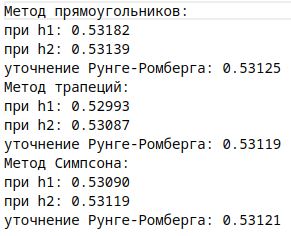
\includegraphics[width=.5\textwidth]{lab3.5}
\caption{Вывод в консоли}
\end{figure}


\subsection{Исходный код}
\lstinputlisting[title=\texttt{3-5.cpp}]{../stud/svoevolin/3-5.cpp}
\pagebreak